\item \defpoints{5} [Convolution layer implementation details]

Check the \href{https://pytorch.org/docs/stable/generated/torch.nn.Conv2d.html#torch.nn.Conv2d}{pytorch document}, point out whether the convolution layer in PyTorch is using cross-correlation or convolution? And why it is defined like this? \defpoints{5}

\solution

From the document, we can see that the convolution layer in PyTorch is using cross-correlation.
\begin{figure}[h]
    \centering
    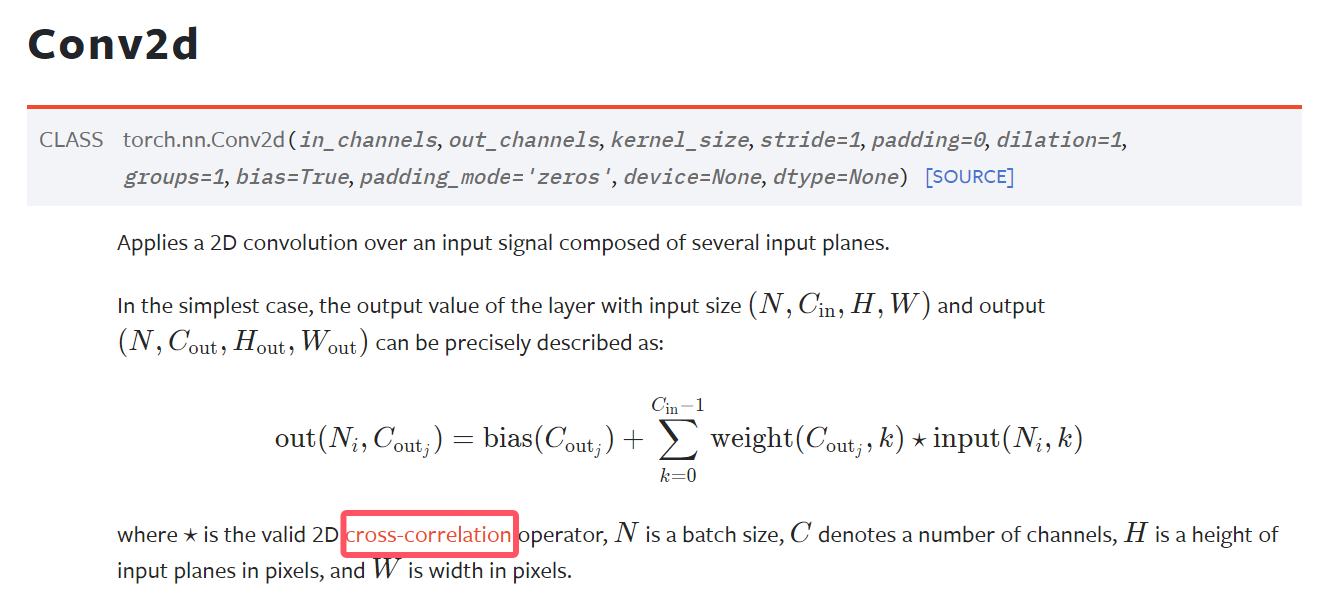
\includegraphics[width=\textwidth]{torch_conv.png}
\end{figure}

The kernel in the convolution layer in PyTorch is learnable, so we don't have to worry about whether it has been flipped or not. Cross-correlation is easier to compute.

\newpage